\documentclass[preprint,12pt,aps,pra,showkeys,amsmath,amssymb,superscriptaddress,floatfix]{revtex4-2}
\usepackage[T1]{fontenc}
\usepackage[utf8]{inputenc}
\usepackage{amsmath,amssymb,amsthm,mathtools,mathrsfs}
\usepackage{microtype,booktabs,enumitem}
\usepackage{xcolor,tikz,etoolbox}
\usepackage[skins,breakable]{tcolorbox}
\usepackage{needspace}
% Keep diagram geometry independent of REVTeX preprint body spacing.
\AtBeginEnvironment{tikzpicture}{\linespread{1}\selectfont}
\usetikzlibrary{arrows.meta,positioning,calc,fit,decorations.pathreplacing}
\usepackage{graphicx}
\usepackage{hyperref}

\definecolor{MMBlue}{RGB}{0,82,155}
\definecolor{MMOrange}{RGB}{200,80,0}
\tikzset{
 mmnode/.style={draw=MMBlue,rounded corners=2pt,fill=MMBlue!4,align=left,execute at begin node={\raggedright},text width=5cm,font=\fontsize{10}{12}\selectfont,inner sep=6pt},
 mmimport/.style={mmnode,draw=black!65,fill=black!4},
 mmcandidate/.style={mmnode,draw=MMOrange,dashed,fill=MMOrange!5},
 mmrejected/.style={mmnode,draw=black,densely dotted,fill=black!8},
 mmproof/.style={->,thick,MMBlue},
 mmflow/.style={->,semithick,black!70},
 mmrepair/.style={->,dashed,thick,MMOrange},
 mmcandidatearrow/.style={->,dashed,semithick,MMOrange},
 mmnote/.style={font=\scriptsize,fill=white,inner sep=2pt,align=center}}

\usepackage[section]{placeins}
\setlength{\emergencystretch}{3em}
\setlist{itemsep=3pt,topsep=4pt}
\newtheorem{theorem}{Theorem}[section]
\newtheorem{proposition}[theorem]{Proposition}
\newtheorem{lemma}[theorem]{Lemma}
\newtheorem{corollary}[theorem]{Corollary}
\theoremstyle{definition}
\newtheorem{definition}[theorem]{Definition}
\newtheorem{example}[theorem]{Example}
\theoremstyle{remark}
\newtheorem{remark}[theorem]{Remark}
% Avoid isolated statement headings and single-line paragraph fragments.
\BeforeBeginEnvironment{theorem}{\Needspace{6\baselineskip}}
\BeforeBeginEnvironment{definition}{\Needspace{5\baselineskip}}
\BeforeBeginEnvironment{proposition}{\Needspace{5\baselineskip}}
\BeforeBeginEnvironment{lemma}{\Needspace{5\baselineskip}}
\BeforeBeginEnvironment{corollary}{\Needspace{5\baselineskip}}
\clubpenalty=5000
\widowpenalty=5000
\newcommand{\R}{\mathbb R}\newcommand{\Z}{\mathbb Z}\newcommand{\N}{\mathbb N}
\newcommand{\Pa}{\operatorname{Pa}}\newcommand{\Desc}{\operatorname{Desc}}
\newcommand{\cl}{\operatorname{cl}}\newcommand{\cost}{\operatorname{cost}}
\newcommand{\status}{\operatorname{status}}
% Faculty cards: a visual rail groups the five faculties within one agent.
% The rail has no arrowhead and does not represent a proof dependency.
\newcommand{\mmfacultybadge}[1]{%
 \node[circle,draw=MMBlue,line width=1pt,fill=white,
 minimum size=7mm,inner sep=0pt,font=\sffamily\small\bfseries,text=MMBlue]
 at ([xshift=15pt,yshift=-15pt]frame.north west) {#1};}
\newcommand{\mmfacultyrail}{%
 \draw[MMBlue!80,line width=1pt]
 ([xshift=15pt,yshift=2pt]frame.north west)--
 ([xshift=15pt,yshift=-2pt]frame.south west);}
\newtcolorbox{mmfacultybox}[2]{enhanced,breakable,
 colback=MMBlue!4,colframe=MMBlue!4,boxrule=0pt,arc=3pt,
 left=39pt,right=9pt,top=4pt,bottom=4pt,
 before skip=2pt,after skip=2pt,
 fontupper=\small\linespread{1.1}\selectfont,
 overlay unbroken={\mmfacultyrail\mmfacultybadge{#1}},
 overlay first={\mmfacultyrail\mmfacultybadge{#1}},
 overlay middle={\mmfacultyrail},overlay last={\mmfacultyrail}}
\newcommand{\mmfaculty}[3]{%
 \begin{mmfacultybox}{#1}{#2}
 {\sffamily\bfseries\color{MMBlue}#2}\par\smallskip #3
 \end{mmfacultybox}}
\newcommand{\agent}[9]{%
 \Needspace{8\baselineskip}
 \subsubsection{#1}
 \noindent\textbf{Object.} #2\par
 \noindent\textbf{Role.} #3\par\smallskip
 \mmfaculty{E}{Ego}{#4}
 \mmfaculty{M}{Memory}{#5}
 \mmfaculty{I}{Intellect}{#6}
 \mmfaculty{S}{Sense}{#7}
 \mmfaculty{A}{Action}{#8}
 \smallskip\noindent #9\par}

\usepackage{longtable,array,calc}
\providecommand{\tightlist}{\setlength{\itemsep}{2pt}\setlength{\parskip}{0pt}}
\makeatletter
\def\frontmatter@abstract@produce{\par\addvspace{\frontmatter@preabstractspace}%
\begingroup\prep@absbox\unvbox\absbox\post@absbox\endgroup
\addvspace{\frontmatter@postabstractspace}}
\makeatother
\newcommand{\field}[2]{\par\smallskip\noindent\textbf{#1.} #2\par}
\setlength{\emergencystretch}{5em}
\AtBeginEnvironment{verbatim}{\small\linespread{1.0}\selectfont}


\hypersetup{colorlinks=true,linkcolor=MMBlue,urlcolor=MMBlue,pdfauthor={Dibakar Sigdel}}

\begin{document}

\title{Urysohn's Lemma\\[4pt]\large An End-to-End Meta-Math Walkthrough}

\author{Dibakar Sigdel}

\affiliation{Mindverse Computing LLC, Lynnwood, WA 98087, USA}

\date{October 2026}

\begin{abstract}

A complete authored walkthrough of urysohn's lemma, with explicit
mathematical contracts, local verification gates, and reusable exports.
The report presents the target theorem, declared imports, a dependency
graph, five-faculty node contracts, a continuous proof, a worked
example, and a hypothesis-repair audit. It is an authored mathematical
exposition, not a deployed-agent transcript or a formal proof-assistant
certificate.

\end{abstract}\maketitle\linespread{1.12}\selectfont

\noindent\textbf{GT-03 / General Topology / Report v1}

\section{Target and import contract}

\begin{theorem}

For a normal \(T_1\) space \(X\) and disjoint closed sets \(A,B\), prove
a continuous \(f:X\to[0,1]\) exists with \(f=0\) on \(A\) and \(f=1\) on
\(B\).

\end{theorem}

\subsection{Foundations and permitted imports}

Normal means every pair of disjoint closed sets has disjoint open
neighborhoods; \(T_{1}\) means points are closed. Under this convention
derive the shrinking lemma below. Dyadic rationals are dense
in{[}0,1{]}. The construction uses closures in X and no metric. EmptyA
or B is allowed.

\clearpage\section{Node interaction workflow}

\begin{center}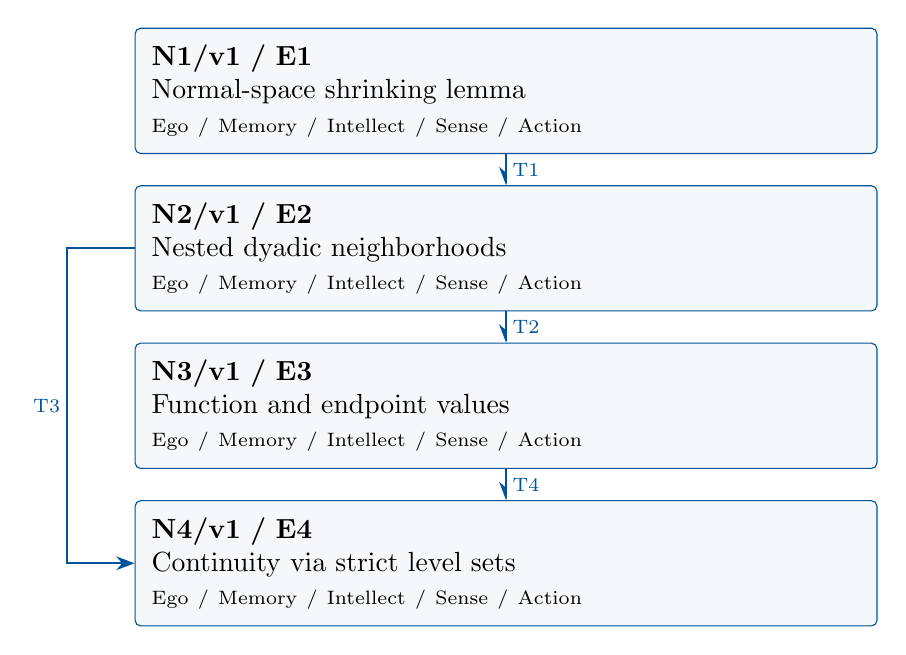
\begin{tikzpicture}[>=Stealth,x=1cm,y=1cm]

\node[mmnode,text width=9cm,minimum height=1.25cm] (N1) at (0,0.0) {\textbf{N1/v1 / E1}\\Normal-space shrinking lemma\\{\scriptsize Ego / Memory / Intellect / Sense / Action}};

\node[mmnode,text width=9cm,minimum height=1.25cm] (N2) at (0,-2.0) {\textbf{N2/v1 / E2}\\Nested dyadic neighborhoods\\{\scriptsize Ego / Memory / Intellect / Sense / Action}};

\node[mmnode,text width=9cm,minimum height=1.25cm] (N3) at (0,-4.0) {\textbf{N3/v1 / E3}\\Function and endpoint values\\{\scriptsize Ego / Memory / Intellect / Sense / Action}};

\node[mmnode,text width=9cm,minimum height=1.25cm] (N4) at (0,-6.0) {\textbf{N4/v1 / E4}\\Continuity via strict level sets\\{\scriptsize Ego / Memory / Intellect / Sense / Action}};

\draw[mmproof] (N1.south) -- node[mmnote,right] {T1} (N2.north);

\draw[mmproof] (N2.south) -- node[mmnote,right] {T2} (N3.north);

\draw[mmproof] (N2.west) -- (-5.58,-2) -- node[mmnote,left] {T3} (-5.58,-6) -- (N4.west);

\draw[mmproof] (N3.south) -- node[mmnote,right] {T4} (N4.north);

\end{tikzpicture}\end{center}

Each box is one mathematical agent containing all five faculties. Blue
arrows carry the versioned exports listed below. The layout gives a
reading order; only drawn arrows assert dependencies. Diagnostic repair
is separate from the proof DAG.

\clearpage\subsection{Versioned evidence-transfer ledger}

\begingroup\small\linespread{1.05}\selectfont

\Needspace{5\baselineskip}\field{T1: N1/E1/v1 to N2}{A neighborhood whose closure stays inside the prescribed open set.}

\field{Receiving activity}{N2: Nested dyadic neighborhoods}

\field{Compatibility}{Use the same mathematical objects and hypotheses as the source export.
Receiving contract: InitialU \(_{0},U_{1}\) and shrinking lemma; prior
exports E1/v1}

\Needspace{5\baselineskip}\field{T2: N2/E2/v1 to N3}{A family with \(\operatorname{closure} (U_r)\subset U_s\) whenever
\(r<s\).}

\field{Receiving activity}{N3: Function and endpoint values}

\field{Compatibility}{Use the same mathematical objects and hypotheses as the source export.
Receiving contract: Nested neighborhoods; prior exports E2/v1}

\Needspace{5\baselineskip}\field{T3: N2/E2/v1 to N4}{A family with \(\operatorname{closure} (U_r)\subset U_s\) whenever
\(r<s\).}

\field{Receiving activity}{N4: Continuity via strict level sets}

\field{Compatibility}{Use the same mathematical objects and hypotheses as the source export.
Receiving contract: Infimum definition and closure nesting; prior
exports E2/v1, E3/v1}

\Needspace{5\baselineskip}\field{T4: N3/E3/v1 to N4}{A function into{[}0,1{]} taking the specified endpoint values.}

\field{Receiving activity}{N4: Continuity via strict level sets}

\field{Compatibility}{Use the same mathematical objects and hypotheses as the source export.
Receiving contract: Infimum definition and closure nesting; prior
exports E2/v1, E3/v1}

\endgroup

\clearpage\section{Agent roles and five-faculty activities}\begingroup\small\linespread{1.05}\selectfont\setlist{itemsep=1pt,topsep=2pt}

\subsection{N1/v1: Normal-space shrinking lemma}

\field{Object and role}{Separate F from the closed complement.}

\field{Inputs}{ClosedF inside open G; foundational imports stated in §1}

\mmfaculty{E}{Ego}{Own E1/v1: A neighborhood whose closure stays inside the prescribed open
set.}

\mmfaculty{M}{Memory}{Retain ClosedF inside open G; foundational imports stated in §1; keep
their assumptions and versions attached.}

\mmfaculty{I}{Intellect}{Separate F from the closed complement.}

\mmfaculty{S}{Sense}{Disjoint open neighborhoods alone are insufficient unless the closure
inclusion is obtained.}

\mmfaculty{A}{Action}{Carry out the numbered deductions and publish E1/v1 together with its
hypotheses and proof location.}

\smallskip\noindent\textbf{Numbered mathematical activities}

\begin{enumerate}[label=N1.\arabic*,leftmargin=3.4em]

\item Normality gives disjoint open U,V containing F and \(X\setminus G\).

\item Since \(U\subset X\setminus V\) and \(X\setminus V\) is closed,
\(\operatorname{closure} (U)\subset X\setminus V\subset G\).

\item Thus \(F\subset U\subset \operatorname{closure} (U)\subset G\).

\item Take \(G=X\setminus B\) and \(F=A\) to choose \(U_{0}\) with
\(A\subset U_{0}\subset \operatorname{closure} (U_{0})\subset U_{1}=X\setminus B\).

\end{enumerate}

\field{Export E1/v1}{A neighborhood whose closure stays inside the prescribed open set.}

\field{Acceptance gate}{Disjoint open neighborhoods alone are insufficient unless the closure
inclusion is obtained. Publish only after checking every displayed
deduction.}

\field{Targeted repair}{If the check fails, revise N1: Disjoint open neighborhoods alone are
insufficient unless the closure inclusion is obtained. Recheck dependent
nodes N2, N3, N4.}

\clearpage

\subsection{N2/v1: Nested dyadic neighborhoods}

\field{Object and role}{Insert midpoint neighborhoods between neighboring dyadics.}

\field{Inputs}{InitialU \(_{0},U_{1}\) and shrinking lemma; prior exports E1/v1}

\mmfaculty{E}{Ego}{Own E2/v1: A family with \(\operatorname{closure} (U_r)\subset U_s\)
whenever \(r<s\).}

\mmfaculty{M}{Memory}{Retain InitialU \(_{0},U_{1}\) and shrinking lemma; prior exports E1/v1;
keep their assumptions and versions attached.}

\mmfaculty{I}{Intellect}{Insert midpoint neighborhoods between neighboring dyadics.}

\mmfaculty{S}{Sense}{Bare \(inclusionsU_r\subset U_s\) do not supply the continuity argument.}

\mmfaculty{A}{Action}{Carry out the numbered deductions and publish E2/v1 together with its
hypotheses and proof location.}

\smallskip\noindent\textbf{Numbered mathematical activities}

\begin{enumerate}[label=N2.\arabic*,leftmargin=3.4em]

\item At each finite dyadic stage, for every consecutive \(pairr<s\) already
constructed choose \(U_{r+s}/2\) using
\(F=\operatorname{closure} (U_r)\subset G=U_s\).

\item Thus
\(\operatorname{closure} (U_r)\subset U_mid\subset \operatorname{closure} (U_mid)\subset U_s\).

\item Induction defines \(U_r\) for all dyadicr \(\in [0,1]\), and for
\(anyr<s\) their levels share a sufficiently fine stage, giving
\(\operatorname{closure} (U_r)\subset U_s\).

\item All \(U_r\) \(withr<1\) lie in \(X\setminus B\).

\end{enumerate}

\field{Export E2/v1}{A family with \(\operatorname{closure} (U_r)\subset U_s\) whenever
\(r<s\).}

\field{Acceptance gate}{Bare \(inclusionsU_r\subset U_s\) do not supply the continuity argument.
Publish only after checking every displayed deduction.}

\field{Targeted repair}{If the check fails, revise N2: Bare \(inclusionsU_r\subset U_s\) do not
supply the continuity argument. Recheck dependent nodes N3, N4.}

\clearpage

\subsection{N3/v1: Function and endpoint values}

\field{Object and role}{Encode membership by an infimum.}

\field{Inputs}{Nested neighborhoods; prior exports E2/v1}

\mmfaculty{E}{Ego}{Own E3/v1: A function into{[}0,1{]} taking the specified endpoint
values.}

\mmfaculty{M}{Memory}{Retain Nested neighborhoods; prior exports E2/v1; keep their assumptions
and versions attached.}

\mmfaculty{I}{Intellect}{Encode membership by an infimum.}

\mmfaculty{S}{Sense}{The empty-infimum convention must be specified.}

\mmfaculty{A}{Action}{Carry out the numbered deductions and publish E3/v1 together with its
hypotheses and proof location.}

\smallskip\noindent\textbf{Numbered mathematical activities}

\begin{enumerate}[label=N3.\arabic*,leftmargin=3.4em]

\item Let \(f(x)=\operatorname{inf} \{r\in D:x\in U_r\}\), taking the value 1
if the set is empty, where D is the set of dyadics in{[}0,1{]}.

\item Then \(0\le f\le 1\).

\item For \(x\in A\), \(x\in U_{0}\), hence \(f=0\).

\item For \(x\in B\) \(noU_r\) containsx, evenU \(_{1}=X\setminus B\), so
\(f=1\).

\end{enumerate}

\field{Export E3/v1}{A function into{[}0,1{]} taking the specified endpoint values.}

\field{Acceptance gate}{The empty-infimum convention must be specified. Publish only after
checking every displayed deduction.}

\field{Targeted repair}{If the check fails, revise N3: The empty-infimum convention must be
specified. Recheck dependent nodes N4.}

\clearpage

\subsection{N4/v1: Continuity via strict level sets}

\field{Object and role}{Prove both types of strict level sets are open.}

\field{Inputs}{Infimum definition and closure nesting; prior exports E2/v1, E3/v1}

\mmfaculty{E}{Ego}{Own E4/v1: The required continuous separator.}

\mmfaculty{M}{Memory}{Retain Infimum definition and closure nesting; prior exports E2/v1,
E3/v1; keep their assumptions and versions attached.}

\mmfaculty{I}{Intellect}{Prove both types of strict level sets are open.}

\mmfaculty{S}{Sense}{Superlevel openness uses closures, not just open neighborhoods.}

\mmfaculty{A}{Action}{Carry out the numbered deductions and publish E4/v1 together with its
hypotheses and proof location.}

\smallskip\noindent\textbf{Numbered mathematical activities}

\begin{enumerate}[label=N4.\arabic*,leftmargin=3.4em]

\item For \(0<a\le 1\), \(\{f<a\}=\cup _{r\in D,r<a}U_r\): membership on
either side follows from the infimum and the existence of a dyadic
membership level belowa.

\item For \(0\le a<1\),
\(\{f>a\}=\cup _{r\in D,a<r<1}(X\setminus\operatorname{cl}(U_r))\).

\item Ifx is outside \(\operatorname{closure} (U_r)\), it belongs to \(noU_s\)
with \(s\le r\), so \(f(x)\ge r>a\).

\item Conversely if \(f(x)>a\) choose \(dyadicsa<r<s<f(x)\), possible even
when \(f=1\).

\item Then \(x\notin U_s\) and \(\operatorname{closure} (U_r)\subset U_s\),
sox lies in that open complement.

\item Level sets outside{[}0,1{]} are trivial.

\item Both strict level types are open, proving continuity and Urysohn's
lemma.

\end{enumerate}

\field{Export E4/v1}{The required continuous separator.}

\field{Acceptance gate}{Superlevel openness uses closures, not just open neighborhoods. Publish
only after checking every displayed deduction.}

\field{Targeted repair}{If the check fails, revise N4: Superlevel openness uses closures, not
just open neighborhoods. Withhold this terminal result until its gate
passes.}

\endgroup\clearpage\section{Continuous mathematical proof}\label{sec:proof}

Read these steps in order as one proof; the diagram is optional.
Numbered activities identify the specific constructions and deductions
owned by each node.

\subsection{§4.N1 --- Normal-space shrinking
lemma}\label{n1-normal-space-shrinking-lemma}

First let \(F\) be closed and \(G\) open with \(F\subset G\).

\begin{enumerate}
\def\labelenumi{\arabic{enumi}.}
\item
  Normality gives disjoint open U,V containing F and \(X\setminus G\).
\item
  Since \(U\subset X\setminus V\) and \(X\setminus V\) is closed,
  \(\operatorname{closure} (U)\subset X\setminus V\subset G\).
\item
  Thus \(F\subset U\subset \operatorname{closure} (U)\subset G\).
\item
  Take \(G=X\setminus B\) and \(F=A\) to choose \(U_{0}\) with
  \(A\subset U_{0}\subset \operatorname{closure} (U_{0})\subset U_{1}=X\setminus B\).
\end{enumerate}

\subsection{§4.N2 --- Nested dyadic
neighborhoods}\label{n2-nested-dyadic-neighborhoods}

\begin{enumerate}
\def\labelenumi{\arabic{enumi}.}
\item
  At each finite dyadic stage, for every consecutive \(pairr<s\) already
  constructed choose \(U_{r+s}/2\) using
  \(F=\operatorname{closure} (U_r)\subset G=U_s\).
\item
  Thus
  \(\operatorname{closure} (U_r)\subset U_mid\subset \operatorname{closure} (U_mid)\subset U_s\).
\item
  Induction defines \(U_r\) for all dyadicr \(\in [0,1]\), and for
  \(anyr<s\) their levels share a sufficiently fine stage, giving
  \(\operatorname{closure} (U_r)\subset U_s\).
\item
  All \(U_r\) \(withr<1\) lie in \(X\setminus B\).
\end{enumerate}

\subsection{§4.N3 --- Function and endpoint
values}\label{n3-function-and-endpoint-values}

\begin{enumerate}
\def\labelenumi{\arabic{enumi}.}
\item
  Let \(f(x)=\operatorname{inf} \{r\in D:x\in U_r\}\), taking the value
  1 if the set is empty, where D is the set of dyadics in{[}0,1{]}.
\item
  Then \(0\le f\le 1\).
\item
  For \(x\in A\), \(x\in U_{0}\), hence \(f=0\).
\item
  For \(x\in B\) \(noU_r\) containsx, evenU \(_{1}=X\setminus B\), so
  \(f=1\).
\end{enumerate}

\subsection{§4.N4 --- Continuity via strict level
sets}\label{n4-continuity-via-strict-level-sets}

\begin{enumerate}
\def\labelenumi{\arabic{enumi}.}
\item
  For \(0<a\le 1\), \(\{f<a\}=\cup _{r\in D,r<a}U_r\): membership on
  either side follows from the infimum and the existence of a dyadic
  membership level belowa.
\item
  For \(0\le a<1\),
  \(\{f>a\}=\cup _{r\in D,a<r<1}(X\setminus\operatorname{cl}(U_r))\).
\item
  Ifx is outside \(\operatorname{closure} (U_r)\), it belongs to
  \(noU_s\) with \(s\le r\), so \(f(x)\ge r>a\).
\item
  Conversely if \(f(x)>a\) choose \(dyadicsa<r<s<f(x)\), possible even
  when \(f=1\).
\item
  Then \(x\notin U_s\) and \(\operatorname{closure} (U_r)\subset U_s\),
  sox lies in that open complement.
\item
  Level sets outside{[}0,1{]} are trivial.
\item
  Both strict level types are open, proving continuity and Urysohn's
  lemma.
\end{enumerate}

\hfill$\square$

\section{Worked orchestration}

In R take \(A=\{0\},B=\{1\}\); a concrete separator is
\(f(x)=\operatorname{max} (0,\operatorname{min} (1,x))\). The dyadic
construction is needed for arbitrary normal spaces; it need not
reproduce this particular function. If A is empty the constant 1 works,
and if B is empty the constant 0 works.

\subsection{Boundary and hypothesis audit}

A candidate drops closure nesting and asserts an arbitrary
membership-threshold function is continuous. Sense identifies that its
superlevel sets may fail to be open. Repair the neighborhood
construction before publishing the function; all later continuity claims
depend on it.

\section{Illustrative failure and repair}

The following is an authored diagnostic scenario. Changed assumptions
define a new contract; they do not retroactively prove the original
statement.

\subsection{Failure and correction}
This is an authored teaching trace, not a recorded agent run.

\begin{enumerate}
\def\labelenumi{\arabic{enumi}.}
\tightlist
\item
  \textbf{Ego \(\to\) Memory:} register the §1 theorem, imports, and
  requested exports before beginning the proof.
\item
  \textbf{Intellect \(\to\) Action:} choose the bridges in §3 and carry
  out the numbered activities in §4; transmit only established E-exports
  along the §2 DAG.
\item
  \textbf{Sense \(\to\) responsible node:} test the specific
  boundary/failure in §5 and the node's individual audit. A failing
  candidate is withheld; downstream nodes may not use it.
\item
  \textbf{Memory + Intellect:} identify whether the error is an omitted
  condition, an invalid inference, or an attempted extension beyond the
  theorem. Restore the exact contract or explicitly state a different
  one.
\item
  \textbf{Action:} redo the affected mathematical activity using the
  repaired condition or inference. Recheck consuming nodes, rather than
  feeding their conclusions back as premises.
\item
  \textbf{Ego:} publish only the supported export with its assumptions
  and proof location. A hypothetical revised export is v2; the written
  proof here is the v1 exposition, not a claim that this repair was
  executed.
\end{enumerate}

\subsection{Hypothesis boundary}
A candidate drops closure nesting and asserts an arbitrary
membership-threshold function is continuous. Sense identifies that its
superlevel sets may fail to be open. Repair the neighborhood
construction before publishing the function; all later continuity claims
depend on it.

\subsection{Version and recheck}
Treat any changed assumption as a new contract. Recheck the revised
export and all of its descendants. A backward diagnostic never
establishes an earlier theorem. This is an authored teaching trace, not
an execution log.

\par\medskip\begingroup\small\linespread{1.0}\selectfont\noindent\textbf{Provenance.} This authored proof is complete relative to its declared imports. Reuse
each export with its assumptions, proof, and version. The original
Markdown remains available for comparison.
\par\endgroup

\par\smallskip\begingroup\small\linespread{1.0}\selectfont\noindent\textbf{Further reading.} \begin{itemize}
\tightlist
\item
  \href{https://ocw.mit.edu/courses/18-901-introduction-to-topology-fall-2004/pages/lecture-notes/}{MIT
  Introduction to Topology: separation, Urysohn, and Tychonoff
  material}.
\end{itemize}\par\endgroup

\end{document}
